\documentclass[aspectratio=169]{beamer}
\usepackage{booktabs}
\usepackage{graphicx}
\usepackage{adjustbox}
\usepackage{amsmath}
% \documentclass[aspectratio=43]{beamer}

% Define `accent`/`accent2` colors for theme customization
\definecolor{accent}{HTML}{006896}
\definecolor{accent2}{HTML}{E64173}

% Beamer theme
% Define colors ----------------------------------------------------------------
\usepackage{xcolor}

\definecolor{purple}{HTML}{695693}
\definecolor{cranberry}{HTML}{E64173}
\definecolor{orange}{HTML}{D65616}
\definecolor{navy}{HTML}{006896}
\definecolor{teal}{HTML}{1A505A}
\definecolor{ruby}{HTML}{9a2515}
\definecolor{alice}{HTML}{107895}
\definecolor{daisy}{HTML}{EBC944}
\definecolor{coral}{HTML}{F26D21}
\definecolor{kelly}{HTML}{829356}
\definecolor{slate900}{HTML}{131516}
\definecolor{asher}{HTML}{555F61}
\definecolor{slate}{HTML}{314F4F}

% Slate from Tailwind Colors
\definecolor{slate50}{HTML}{f8fafc}
\definecolor{slate100}{HTML}{f1f5f9}
\definecolor{slate200}{HTML}{e2e8f0}
\definecolor{slate300}{HTML}{cbd5e1}
\definecolor{slate400}{HTML}{94a3b8}
\definecolor{slate500}{HTML}{64748b}
\definecolor{slate600}{HTML}{475569}
\definecolor{slate700}{HTML}{334155}
\definecolor{slate800}{HTML}{1e293b}
\definecolor{slate900}{HTML}{0f172a}
\definecolor{slate950}{HTML}{020617}

% Easily color text
\newcommand\purple[1]{{\color{purple}#1}}
\newcommand\cranberry[1]{{\color{cranberry}#1}}
\newcommand\orange[1]{{\color{orange}#1}}
\newcommand\navy[1]{{\color{navy}#1}}
\newcommand\teal[1]{{\color{teal}#1}}
\newcommand\kelly[1]{{\color{kelly}#1}}
\newcommand\ruby[1]{{\color{ruby}#1}}
\newcommand\alice[1]{{\color{alice}#1}}
\newcommand\daisy[1]{{\color{daisy}#1}}
\newcommand\coral[1]{{\color{coral}#1}}

% Color background of text
\newcommand\bgNavy[1]{{\colorbox{navy!80!white}{#1}}}
\newcommand\bgOrange[1]{{\colorbox{orange!80!white}{#1}}}
\newcommand\bgTeal[1]{{\colorbox{teal!80!white}{#1}}}
\newcommand\bgPurple[1]{{\colorbox{purple!80!white}{#1}}}
\newcommand\bgKelly[1]{{\colorbox{kelly!80!white}{#1}}}
\newcommand\bgRuby[1]{{\colorbox{ruby!80!white}{#1}}}
\newcommand\bgAlice[1]{{\colorbox{alice!80!white}{#1}}}
\newcommand\bgDaisy[1]{{\colorbox{daisy!80!white}{#1}}}
\newcommand\bgCoral[1]{{\colorbox{coral!80!white}{#1}}}
\newcommand\bgCranberry[1]{{\colorbox{cranberry!80!white}{#1}}}

% Beamer Options ---------------------------------------------------------------

% Background
\setbeamercolor{background canvas}{bg = white}

% Change text margins
\setbeamersize{text margin left = 15pt, text margin right = 15pt} 

% \alert
\setbeamercolor{alerted text}{fg = accent2}

% Frame title
\setbeamercolor{frametitle}{bg = white, fg = slate900}
\setbeamercolor{framesubtitle}{bg = white, fg = accent}
\setbeamerfont{framesubtitle}{size = \small, shape = \itshape}

% Page numbering
\usepackage{appendixnumberbeamer}
\setbeamercolor{page number in head/foot}{fg=slate600}
\setbeamertemplate{footline}[frame number]

% Table of Contents
\setbeamercolor{section in toc}{fg = slate700}
\setbeamercolor{subsection in toc}{fg = slate900}

% Button 
\setbeamercolor{button}{bg = white, fg = slate900}
\setbeamerfont{button}{}
\setbeamercolor{button border}{fg = accent}

% Remove navigation symbols
\setbeamertemplate{navigation symbols}{}

% Table and Figure captions
\setbeamercolor{caption}{fg = slate900!70!white}
\setbeamercolor{caption name}{fg=slate900}
\setbeamerfont{caption name}{shape = \itshape}

% Links
\usepackage{hyperref}
\hypersetup{
  colorlinks = true,
  linkcolor = accent2,
  filecolor = accent2,
  urlcolor = accent2,
  citecolor = accent2,
}

% Line spacing
\usepackage{setspace}
\setstretch{1.3}

% Remove annoying over-full box warnings
\vfuzz2pt 
\hfuzz2pt


% Title page -------------------------------------------------------------------
\setbeamercolor{title}{fg = slate900}
\setbeamercolor{subtitle}{fg = accent}

%% Custom \maketitle and \titlepage
\setbeamertemplate{title page}
{
  %\begin{centering}
  \vspace{20mm}
  {\Large \usebeamerfont{title}\usebeamercolor[fg]{title}\inserttitle}\\ \vskip0.25em%
  \ifx\insertsubtitle\@empty%
  \else%
    {\usebeamerfont{subtitle}\usebeamercolor[fg]{subtitle}\insertsubtitle\par}%
  \fi% 
  {\vspace{10mm}\insertauthor}\\
  {\color{asher}\small{\insertdate}}\\
  %\end{centering}
}

% Table of Contents with Sections ----------------------------------------------
\setbeamerfont{myTOC}{series=\bfseries, size=\Large}
\AtBeginSection[]{
  \begin{frame}{Roadmap}
    \tableofcontents[current]   
  \end{frame}
}

% Block ------------------------------------------------------------------------
\usepackage{tcolorbox}

\defbeamertemplate{block begin}{framed}[1][] {
  \begin{tcolorbox}[colback=slate50, colframe=slate200, arc=0mm]
  {
    \vskip\smallskipamount%
    \ifthenelse{\equal{#1}{}}{}{%
      \raggedright\usebeamerfont*{block title}\usebeamercolor[fg]{title}%
      \textbf{\insertblocktitle}%
      \vskip\medskipamount%
    }
  }%
  \raggedright%
  \usebeamerfont{block body}%
}
\defbeamertemplate{block end}{framed}[1][] {
  \vskip\smallskipamount\end{tcolorbox}
}
\setbeamertemplate{blocks}[framed]

% Colors from plugging base color into https://uicolors.app/create
\usepackage{ifthen}
\newenvironment*{slateBlock}[1]{%
  \begin{tcolorbox}[colback=slate50, colframe=slate200, arc=0mm]{
    \vskip\smallskipamount%
    \ifthenelse{\equal{#1}{}}{}{%
      \raggedright\usebeamerfont*{block title}\usebeamercolor[fg]{title}%
      \textbf{#1}%
      \vskip\medskipamount%
    }%
  }%
  \raggedright%
  \usebeamerfont{block body}%
}{%
  \vskip\smallskipamount\end{tcolorbox}
}

\definecolor{purple50}{HTML}{f9f8fc}
\definecolor{purple100}{HTML}{f1eff8}
\definecolor{purple200}{HTML}{e6e2f2}
\newenvironment*{purpleBlock}[1]{%
  \begin{tcolorbox}[colback=purple50, colframe=purple200, arc=0mm]{
    \vskip\smallskipamount%
    \ifthenelse{\equal{#1}{}}{}{%
      \raggedright\usebeamerfont*{block title}\usebeamercolor[fg]{title}%
      \textbf{#1}%
      \vskip\medskipamount%
    }%
  }%
  \raggedright%
  \usebeamerfont{block body}%
}{%
  \vskip\smallskipamount\end{tcolorbox}
}

\definecolor{cranberry50}{HTML}{fdf2f6}
\definecolor{cranberry100}{HTML}{fbe8ef}
\definecolor{cranberry200}{HTML}{fad0e0}
\newenvironment*{cranberryBlock}[1]{%
  \begin{tcolorbox}[colback=cranberry50, colframe=cranberry200, arc=0mm]{
    \vskip\smallskipamount%
    \raggedright\usebeamerfont*{block title}\usebeamercolor[fg]{title}%
    \textbf{#1}%
  }%
  \vskip\medskipamount%
  \raggedright%
  \usebeamerfont{block body}%
}{%
  \vskip\smallskipamount\end{tcolorbox}
}

% Bullet points ----------------------------------------------------------------

%% Fix left-margins
\settowidth{\leftmargini}{\usebeamertemplate{itemize item}}
\addtolength{\leftmargini}{\labelsep}

%% enumerate item color
\setbeamercolor{enumerate item}{fg = slate600}
\setbeamerfont{enumerate item}{size = \small}
\setbeamertemplate{enumerate item}{\insertenumlabel.}

%% itemize
\setbeamercolor{itemize item}{fg = slate600}
\setbeamerfont{itemize item}{size = \small}
\setbeamertemplate{itemize item}[circle]

%% right arrow for subitems
\setbeamercolor{itemize subitem}{fg = slate600}
\setbeamerfont{itemize subitem}{size = \small}
\setbeamertemplate{itemize subitem}{$\rightarrow$}

\setbeamercolor{itemize subsubitem}{fg = slate600}
\setbeamerfont{itemize subsubitem}{size = \small}
\setbeamertemplate{itemize subsubitem}[square]

% References -------------------------------------------------------------------

%% Bibliography Font, roughly matching aea
\setbeamerfont{bibliography item}{size = \footnotesize}
\setbeamerfont{bibliography entry author}{size = \footnotesize, series = \bfseries}
\setbeamerfont{bibliography entry title}{size = \footnotesize}
\setbeamerfont{bibliography entry location}{size = \footnotesize, shape = \itshape}
\setbeamerfont{bibliography entry note}{size = \footnotesize}

\setbeamercolor{bibliography item}{fg = slate900}
\setbeamercolor{bibliography entry author}{fg = accent!60!slate900}
\setbeamercolor{bibliography entry title}{fg = slate900}
\setbeamercolor{bibliography entry location}{fg = slate900}
\setbeamercolor{bibliography entry note}{fg = slate900}

%% Remove bibliography symbol in slides
\setbeamertemplate{bibliography item}{}


% \begin{columns} --------------------------------------------------------------
\usepackage{multicol}


% Fonts ------------------------------------------------------------------------
% Beamer Option to use custom fonts
\usefonttheme{professionalfonts}

% \usepackage[utopia, smallerops, varg]{newtxmath}
% \usepackage{utopia}
\usepackage[sfdefault,light]{roboto}

% Small adjustments to text kerning
\usepackage{microtype}

% For \underbracket/\overbracket
\usepackage{mathtools}

% References -------------------------------------------------------------------
\usepackage[
    citestyle= authoryear,
    style = authoryear,
    natbib = true, 
    backend = biber
]{biblatex}

% Smaller font-size for references
\renewcommand*{\bibfont}{\small}

% Remove "In:"
\renewbibmacro{in:}{}

% Color citations for slides 
\newenvironment{citecolor}
    {\footnotesize\begin{color}{accent2}}
    {\end{color}}

\newcommand{\citetcolor}[1]{{\footnotesize\textcolor{gray}{\citet{#1}}}}
\newcommand{\citepcolor}[1]{{\footnotesize\textcolor{gray}{\citep{#1}}}}

% Tables -----------------------------------------------------------------------

% When tables are too big, use adjustbox
% \begin{adjustbox}{width = 1.2\textwidth, center}
\usepackage{adjustbox}
\usepackage{array}
\usepackage{threeparttable, booktabs, adjustbox}
    
% Fix \input with tables
% \input fails when \\ is at end of external .tex file
\makeatletter
\let\input\@@input
\makeatother

% Tables too narrow
% \begin{tabularx}{\linewidth}{cols}
% col-types: X - center, L - left, R -right
% Relative scale: >{\hsize=.8\hsize}X/L/R
\usepackage{tabularx}
\newcolumntype{L}{>{\raggedright\arraybackslash}X}
\newcolumntype{R}{>{\raggedleft\arraybackslash}X}
\newcolumntype{C}{>{\centering\arraybackslash}X}

% Table Highlighting -----------------------------------------------------------
% Create top-left and bottom-right markets in tabular cells with a unique matching id and these commands will outline those cells
\usepackage[beamer,customcolors]{hf-tikz}
\usetikzlibrary{calc}
\usetikzlibrary{fit,shapes.misc}

% To set the hypothesis highlighting boxes red.
\newcommand\marktopleft[1]{%
    \tikz[overlay,remember picture] 
        \node (marker-#1-a) at (0,1.5ex) {};%
}
\newcommand\markbottomright[1]{%
    \tikz[overlay,remember picture] 
        \node (marker-#1-b) at (0,0) {};%
    \tikz[accent!80!slate900, ultra thick, overlay, remember picture, inner sep=4pt]
        \node[draw, rectangle, fit=(marker-#1-a.center) (marker-#1-b.center)] {};%
}

% Figures ----------------------------------------------------------------------

% \imageframe{img_name}
% from https://github.com/mattslate900well/cousteau
\newcommand{\imageframe}[1]{%
    \begin{frame}[plain]
        \begin{tikzpicture}[remember picture, overlay]
            \node[at = (current page.center), xshift = 0cm] (cover) {%
                \includegraphics[keepaspectratio, width=\paperwidth, height=\paperheight]{#1}
            };
        \end{tikzpicture}
    \end{frame}%
}

% subfigures
\usepackage{subfigure}

% Highlight slide --------------------------------------------------------------
% \begin{transitionframe} Text \end{transitionframe}
% from paulgp's beamer tips
\newenvironment{transitionframe}{
    \setbeamercolor{background canvas}{bg=accent!60!black}
    \begin{frame}\color{white}\LARGE\centering
}{
    \end{frame}
}



% Title --------------------------------------------
\title{CU Denver Math Camp - Limits \& Derivatives}
\subtitle{Day 1}
\date{August 5, 2024}
\author{Michael R. Karas}

\begin{document}

% ------------------------------------------------------------------------------
\begin{frame}
\maketitle

% \vspace{2.5mm}
{\footnotesize University of Colorado, Boulder}
\end{frame}
% ------------------------------------------------------------------------------

%------------------------------------------------------------------------------
\begin{frame}{About Me}\label{main1}
Michael Karas, PhD Candidate at CU Boulder
\begin{itemize}
	\begin{itemize}
		\item michael.karas@colorado.edu
		\item Entering my 4th year
	\end{itemize}
	\item Economic History, Industrial Organization, Applied Micro
	\begin{itemize}
		\item Manufactured Gas Utility Industry in the early 20th Century
			\begin{itemize}
				\item Responses to regulatory changes, development of block pricing, role of incumbent firms
			\end{itemize}
		\item Do individuals update their political preferences after experiencing a climate change-affected event?
		\item How the development of highways in the 20th century shaped population and economic growth.
	\end{itemize}
	\item Teaching: Intermediate Micro Principles of Macro
	\item Hobbies: Cycling, Skiing
\end{itemize}

\end{frame}
%------------------------------------------------------------------------------


%------------------------------------------------------------------------------
\begin{frame}{Getting to Know Each Other}\label{main1}
\begin{itemize}
	\item{Name}
	\item{Hometown}
	\item{Interests in Economics}
	\item{Hobbies or something about yourself}
\end{itemize}

\end{frame}
%------------------------------------------------------------------------------

%------------------------------------------------------------------------------
\begin{frame}{Grad School Advice}\label{main1}
\begin{itemize}
	\item It will be challenging
	\begin{itemize}
		\item Everyone struggles, even the ``top" students
		\item It may take a while to master the material, probably won't grasp everything on the first attempt
	\item What matters is determination, discipline, and consistency: put the time in and the results will come
	\item Treat it like a job
\end{itemize}
	\item Study Tips
	\begin{itemize}
	\item Practice makes perfect: get old homework/exam from upper students
	\item Study with each other
	\item Recognize when diminishing marginal returns start to set in and take a break
	\end{itemize}
	\item Don't neglect your mental health.  It's okay to take breaks.
	\begin{itemize}
		\item Have fun! CO is a great place, develop a life outside of school
	\end{itemize}
	\end{itemize}
\end{itemize}

\end{frame}
%------------------------------------------------------------------------------

%------------------------------------------------------------------------------
\begin{frame}{Day 1 Topics}\label{main1}
\begin{itemize}
	\begin{itemize}
		\item Limits
		\item Limit Rules
		\item Derivative Definition
		\item Derivative Rules
		\item Natural Log and Exponent Rules
		\item Higher-order Derivatives
	\end{itemize}
\end{itemize}

\end{frame}
%------------------------------------------------------------------------------

%------------------------------------------------------------------------------
\begin{frame}{Limits}\label{main1}
	The limit of \( f(x) \) as \( x \) approaches \( a \) is written as:
\[
\lim_{x \to a} f(x)
\]
\begin{itemize}
\begin{itemize}
	\item The behavior of the function as its input approaches \( a \)
	\item In certain cases, can be evaluated by plugging in \( x = a \)
	\item \( \lim_{x \to a} c = c \) for a constant \( c \)
	\item \(\lim_{x \to a} x = a \) for a constant \( c \)
\end{itemize}
\end{itemize}

\end{frame}
%------------------------------------------------------------------------------

%------------------------------------------------------------------------------
\begin{frame}{Limits}\label{main1}
The limit from the left and right are
\begin{itemize}
\begin{itemize}
    \item \(\lim_{x \to a^-} f(x) = A\) “as \(x\) approaches \(a\) from the left (\(-\infty\))”
    \item \(\lim_{x \to a^+} f(x) = A\) “as \(x\) approaches \(a\) from the right (\(\infty\))”
\end{itemize}
\end{itemize}
If \(\lim_{x \to a^-} f(x) = A = \lim_{x \to a^+} f(x)\) then the limit exists and we write
\[
\lim_{x \to a} f(x) = A
\]
\begin{itemize}
    \item Note: the limit does not exist if \(A = \pm\infty\), even if the left and right limit both equal \(\pm\infty\)
\end{itemize}
\end{frame}
%------------------------------------------------------------------------------

%------------------------------------------------------------------------------
\begin{frame}{Limits}\label{main1}
    \begin{figure}
        \centering
        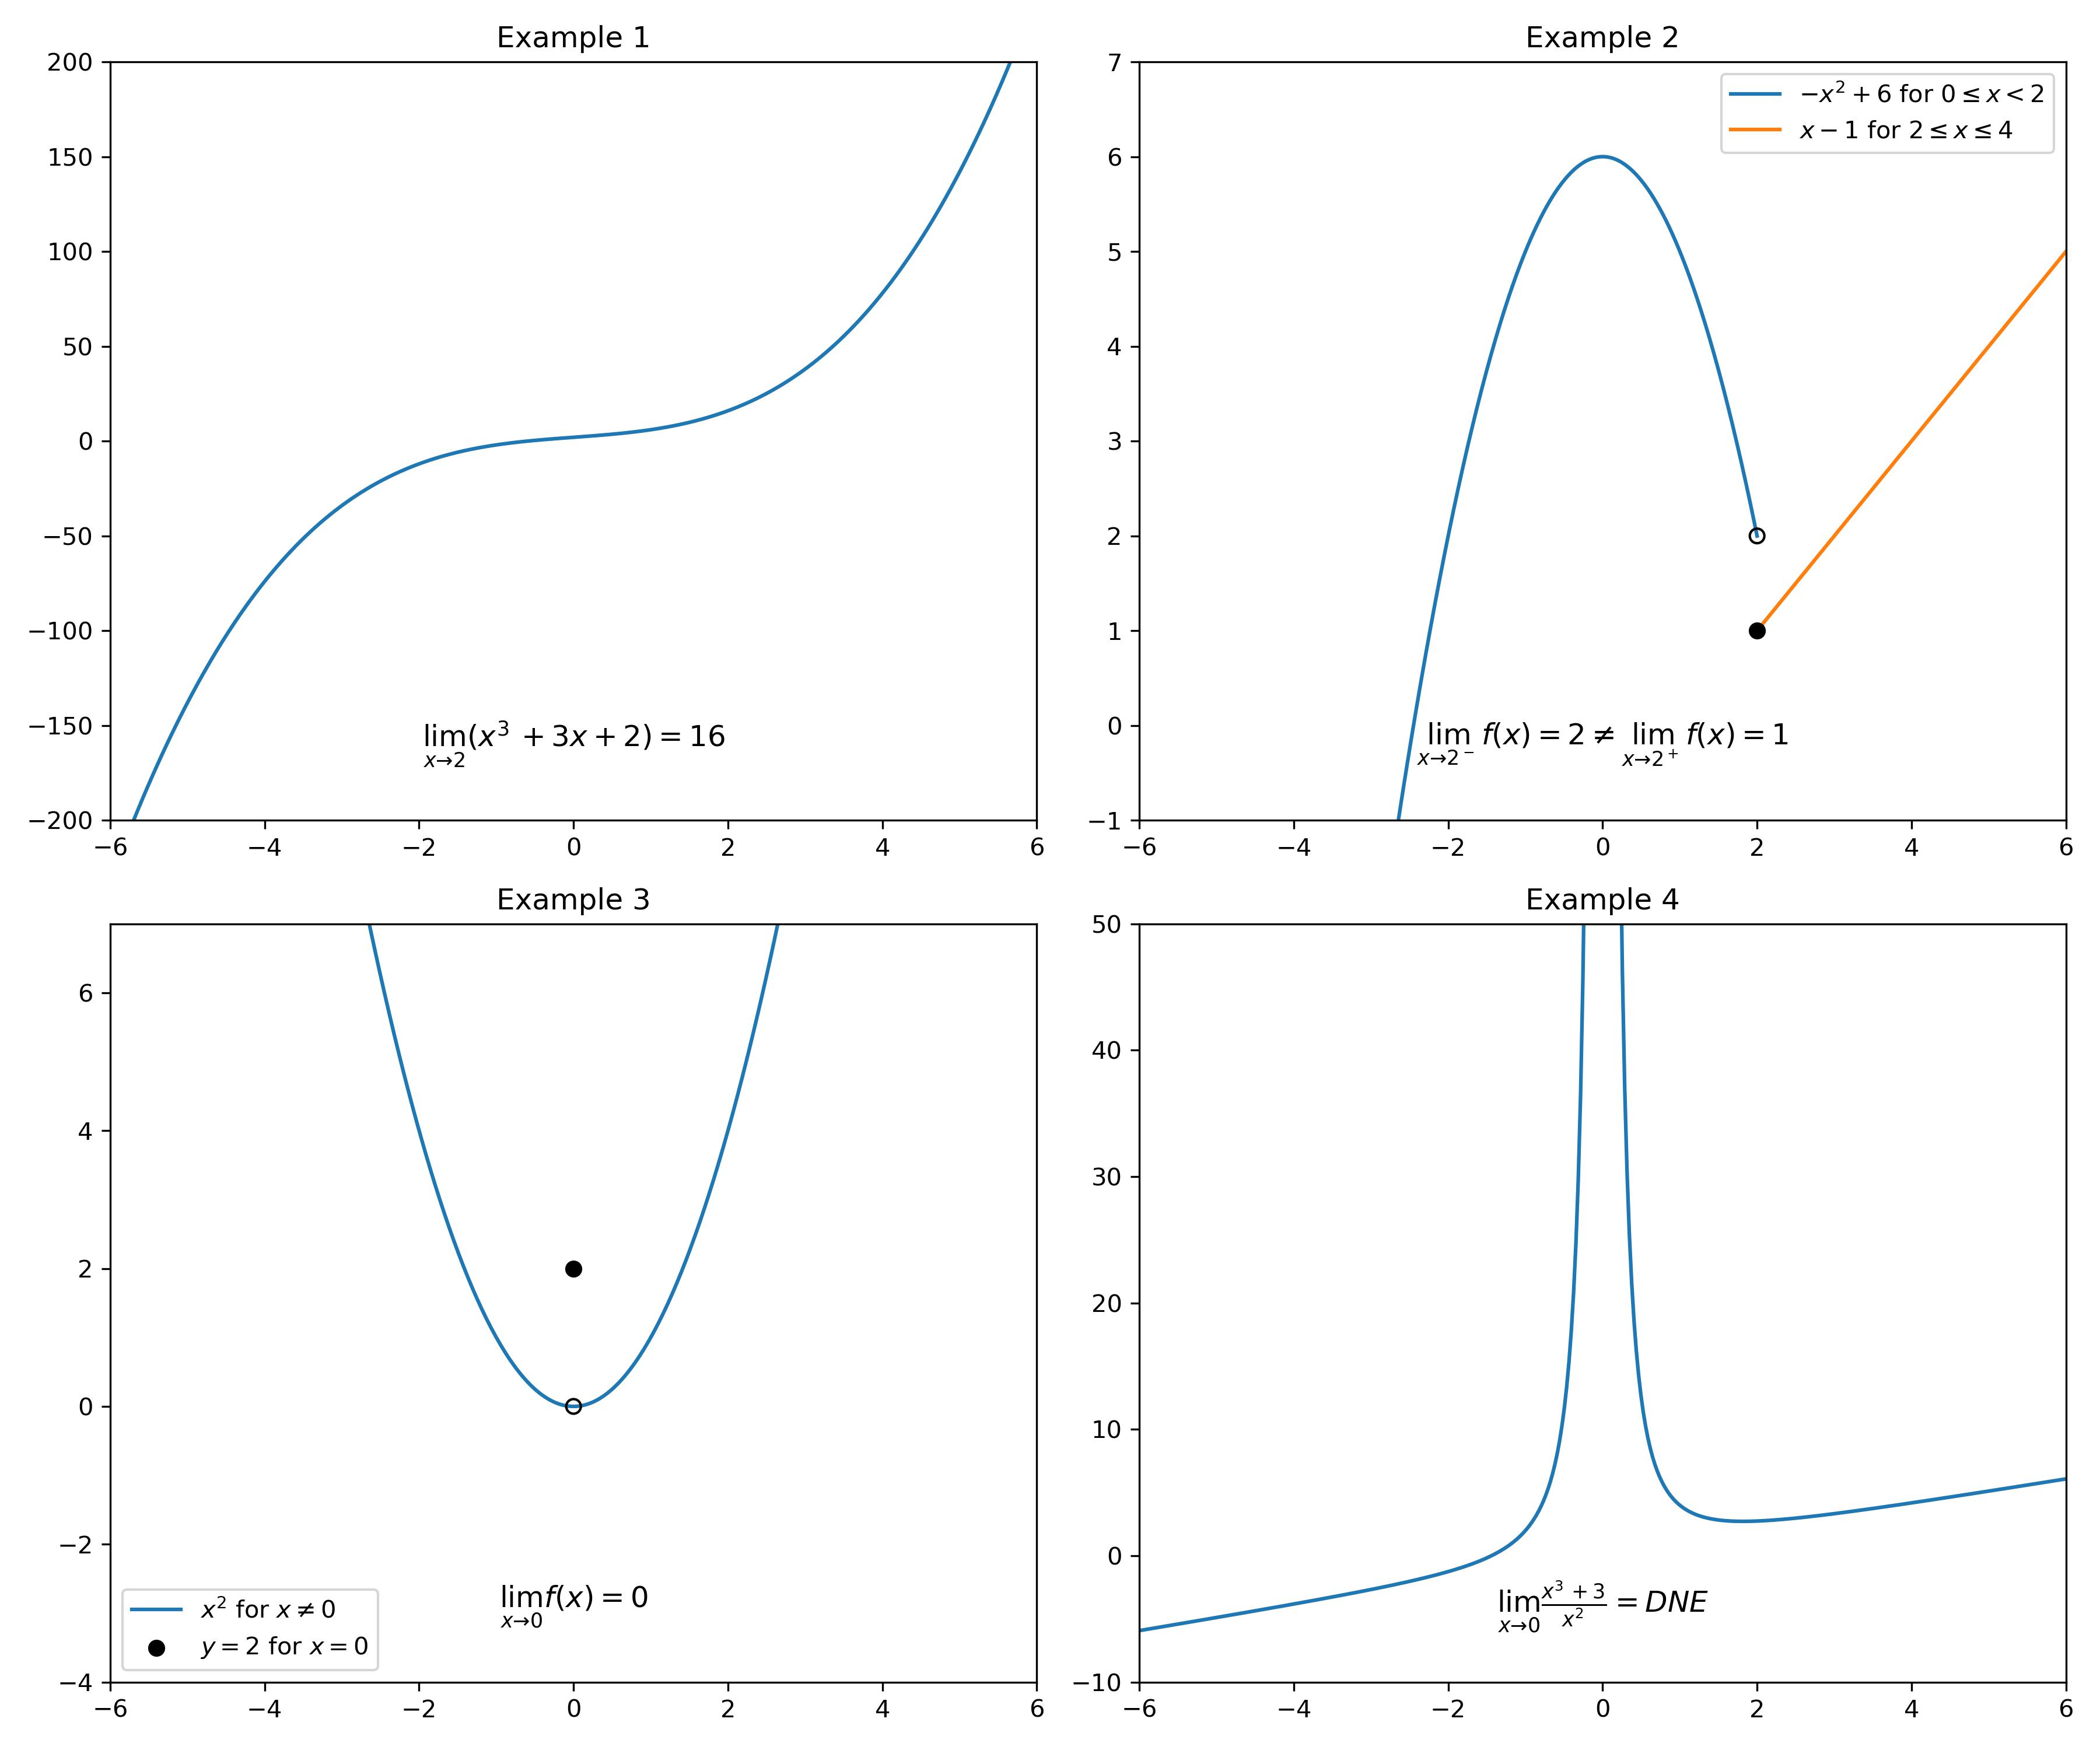
\includegraphics[width=0.6\textwidth]{/Users/michaelkaras/Documents/CU_Denver_Math_Camp/limits_example.jpg}
    \end{figure}
\end{frame}
%------------------------------------------------------------------------------

%------------------------------------------------------------------------------
\begin{frame}{Limit Rules}\label{main1}
    \[
    \lim_{x \to a} f(x) = L \quad \lim_{x \to a} g(x) = M
    \]
    \vspace{1em}
    \begin{itemize}
        \item \textbf{Constant Multiple Rule:} \quad $\lim_{x \to a} [a f(x)] = a L$
        \item \textbf{Sum/Difference Rule:} \quad $\lim_{x \to a} [f(x) \pm g(x)] = L \pm M$
        \item \textbf{Product Rule:} \quad $\lim_{x \to a} [f(x) \cdot g(x)] = L \cdot M$
        \item \textbf{Quotient Rule:} \quad $\lim_{x \to a} \left[ \frac{f(x)}{g(x)} \right] = \frac{L}{M}, \quad M \neq 0$
        \item \textbf{Power Rule:} \quad $\lim_{x \to a} [(f(x))^n] = L^n, \quad n > 0$
    \end{itemize}
\end{frame}
%------------------------------------------------------------------------------

%------------------------------------------------------------------------------
\begin{frame}{Limit Practice Problems}\label{main1}
    \vspace{-4cm}
    \[
    \lim_{x \to 0} (3 + 2x^{2})
    \]
\end{frame}
%------------------------------------------------------------------------------

%------------------------------------------------------------------------------
\begin{frame}{Limit Practice Problems}\label{main1}
	\vspace{-4cm}
    \[
    \lim_{x \to 1} \frac{x^{2} + 7x - 8}{x - 1} 
    \]
\end{frame}
%------------------------------------------------------------------------------

%------------------------------------------------------------------------------
\begin{frame}{Definition of a Derivative}\label{main1}
The derivative of \(f\) is defined as
\[
f'(x) = \lim_{h \to 0} \frac{f(x + h) - f(x)}{h}
\]
If this limit exists, then we say \(f\) is differentiable at \(x\).
\begin{itemize}
	\begin{itemize}
    \item Find \(f(x + h)\). Ex: \(f(x) = x^2\), \(f(x + h) = (x + h)^2 = x^2 + 2xh + h^2\)
    \item Find \(f(x + h) - f(x)\)
    \item Find \(\frac{f(x + h) - f(x)}{h}\) and simplify until \(h = 0\) doesn’t divide by 0
    \item Plug-in \(h = 0\) to determine the limit
    \end{itemize}
\end{itemize}
\end{frame}
%------------------------------------------------------------------------------

%------------------------------------------------------------------------------
\begin{frame}{Definition of a Derivative Practice Problems}\label{main1}
	\vspace{-4cm}
    \[
    f(x) = x^{2}
    \]
\end{frame}
%------------------------------------------------------------------------------

%------------------------------------------------------------------------------
\begin{frame}{Derivative Notation}\label{main1}
All of these mean “take the derivative of \(f\) with respect to \(x\)”:
\begin{itemize}
\begin{itemize}
    \item \(f'(x)\)
    \item \(\frac{df(x)}{dx}\)
    \item \(\frac{d}{dx} f(x)\)
    \item \(\frac{dy}{dx}\) if \(y = f(x)\)
    \item \(y'\) (sometimes)
    \item \( \dot{y} \) (particularly in Macro)
\end{itemize}
\end{itemize}
\end{frame}
%------------------------------------------------------------------------------

%------------------------------------------------------------------------------
\begin{frame}{Derivative Rules}\label{main1}
Let \(f(x)\) and \(g(x)\) be differentiable functions:
\begin{itemize}
    \item \textbf{Derivative of a Constant:} \(f(x) = c\), \(f'(x) = 0\)
    \item \textbf{“Power Rule”:} \(f(x) = x^n\), \(f'(x) = nx^{n-1}\) 
    \item \textbf{Sum/Difference Rule:} \quad $\frac{d}{dx} [f(x) \pm g(x)] = f'(x) \pm g'(x)$
    \item \textbf{Product Rule:} \quad $\frac{d}{dx} [f(x) \cdot g(x)] = f'(x) \cdot g(x) + f(x) \cdot g'(x)$
    \item \textbf{Quotient Rule:} \quad $\frac{d}{dx} \left( \frac{f(x)}{g(x)} \right) = \frac{f'(x) \cdot g(x) - f(x) \cdot g'(x)}{[g(x)]^2}$
    \item \textbf{Chain Rule:} \quad $\frac{d}{dx} f(g(x)) = f'(g(x)) \cdot g'(x)$
\end{itemize}
\end{frame}
%------------------------------------------------------------------------------

%------------------------------------------------------------------------------
\begin{frame}{Derivative Practice Problems}\label{main1}
	\vspace{-4cm}
    \[
    f(x) = 9x^{10}
    \]
\end{frame}
%------------------------------------------------------------------------------

%------------------------------------------------------------------------------
\begin{frame}{Derivative Practice Problems}\label{main1}
	\vspace{-4cm}
    \[
    f(x) = 8x^{4} + 2 \sqrt{x}
    \]
\end{frame}
%------------------------------------------------------------------------------

%------------------------------------------------------------------------------
\begin{frame}{Derivative Practice Problems}\label{main1}
	\vspace{-4cm}
    \[
    f(x) = \sqrt{x} * 6x^{4}
    \]
\end{frame}
%------------------------------------------------------------------------------

%------------------------------------------------------------------------------
\begin{frame}{Derivative Practice Problems}\label{main1}
	\vspace{-4cm}
    \[
    f(x) = \frac{x + 1}{x - 1}
    \]
\end{frame}
%------------------------------------------------------------------------------

%------------------------------------------------------------------------------
\begin{frame}{Derivative Practice Problems}\label{main1}
	\vspace{-4cm}
    \[
    f(x) = 5u^{4} ; u = 1 + x^{2}
    \]
\end{frame}
%------------------------------------------------------------------------------

%------------------------------------------------------------------------------
\begin{frame}{Properties of Exponents}\label{main1}
Let $a$ and $b$ be real numbers and $m$ and $n$ be integers. Then the following properties of exponents hold, provided that all of the expressions appearing in a particular equation are defined:
\begin{itemize}
\begin{itemize}
    \item $a^m a^n = a^{m+n}$
    \item $(a^m)^n = a^{mn}$
    \item $(ab)^m = a^m b^m$
    \item $\frac{a^m}{a^n} = a^{m-n}$, $a \neq 0$
    \item $\left(\frac{a}{b}\right)^m = \frac{a^m}{b^m}$, $b \neq 0$
    \item $a^{-m} = \frac{1}{a^m}$, $a \neq 0$
    \item $a^{\frac{1}{n}} = \sqrt[n]{a}$
    \item $a^0 = 1$, $a \neq 0$
    \item $a^{\frac{m}{n}} = \sqrt[n]{a^m} = \left(\sqrt[n]{a}\right)^m$
\end{itemize}
\end{itemize}
\end{frame}
%------------------------------------------------------------------------------

%------------------------------------------------------------------------------
\begin{frame}{Derivative Practice Problems}\label{main1}
	\vspace{-4cm}
    \[
    f(x) = \frac{x + 1}{x^{5}}
    \]
\end{frame}
%------------------------------------------------------------------------------

%------------------------------------------------------------------------------
\begin{frame}{Properties of Natural Log}\label{main1}
Note that logs are only defined for positive values of x:
\begin{itemize}
\begin{itemize}
    \item $\ln(xy) = \ln(x) + \ln(y)$
    \item $\ln\left(\frac{x}{y}\right) = \ln(x) - \ln(y)$
    \item $\ln(x^y) = y \cdot \ln(x)$
    \item $\ln(e^x) = x$
    \item $e^{\ln(x)} = x$
    \item $\ln(e) = 1$
    \item $\ln(1) = 0$
    \item $\ln(1) = undefined$
\end{itemize}
\end{itemize}
\end{frame}
%------------------------------------------------------------------------------

%------------------------------------------------------------------------------
\begin{frame}{Derivative Rules for Exponents and Natural Log}\label{main1}
\begin{itemize}
\begin{itemize}
    \item \(f(x) = e^x\), \(f'(x) = e^x\)
    \item \(f(x) = \ln(x)\), \(f'(x) = \frac{1}{x}\)
\end{itemize}
\end{itemize}
\end{frame}
%------------------------------------------------------------------------------

%------------------------------------------------------------------------------
\begin{frame}{Natural Log/Exponent Derivative Practice Problems}\label{main1}
	\vspace{-4cm}
    \[
    f(x) = 3x^{2}*ln(x)
    \]
\end{frame}
%------------------------------------------------------------------------------


%------------------------------------------------------------------------------
\begin{frame}{Natural Log/Exponent Derivative Practice Problems}\label{main1}
	\vspace{-4cm}
    \[
    f(x) = x^{4}*e^{x}
    \]
\end{frame}
%------------------------------------------------------------------------------

%------------------------------------------------------------------------------
\begin{frame}{Natural Log/Exponent Derivative Practice Problems}\label{main1}
	\vspace{-4cm}
    \[
    f(x) = e^{x}*(1-x)^{4}
    \]
\end{frame}
%------------------------------------------------------------------------------

%------------------------------------------------------------------------------
\begin{frame}{Higher-order Derivatives}\label{main1}
The second-order derivative is

\[
f''(x) = \frac{d}{dx} f'(x)
\]

We could keep differentiating as long as the last derivative is differentiable. Notation:
\begin{itemize}
\begin{itemize}
    \item $f''(x)$
    \item $\frac{d^2 f(x)}{dx^2}$
    \item $\frac{d^2}{dx^2} f(x)$
    \item $\frac{d^2 y}{dx^2}$ if $y = f(x)$
    \item $y''$ (sometimes)
\end{itemize}
\end{itemize}
\end{frame}
%------------------------------------------------------------------------------

%------------------------------------------------------------------------------
\begin{frame}{Topics for Tomorrow}\label{main1}

\begin{itemize}
	\begin{itemize}
		\item Increasing/Decreasing Functions
		\item Concave/Convex Functions
		\item Implicit Differentiation
		\item Partial Derivatives
		\item Taylor Series
	\end{itemize}
\end{itemize}
\end{frame}
%------------------------------------------------------------------------------

\end{document}
